\documentclass[pdf]{beamer}
%\mode<presentation>{}

\usepackage{amssymb,amsmath,amsthm,enumerate,mathtools}
\usepackage[utf8]{inputenc}
\usepackage{array}
\newcolumntype{C}[1]{>{\centering\arraybackslash}m{#1}}

\usepackage[parfill]{parskip}
\usepackage{graphicx}
\usepackage{caption}
\captionsetup[figure]{labelformat=empty}
\usepackage{subcaption}
\usepackage{bm}
\usepackage{amsfonts,amscd}
%\usepackage{gensymb}
\usepackage[]{units}
\usepackage{listings}
\usepackage{multicol}
\usepackage{tcolorbox}
\usepackage{physics}
\usepackage{multirow}
\usepackage{pgfplots,tikz}
\pgfplotsset{compat=1.7}
\usepackage{hyperref}
\hypersetup{
    colorlinks=true,
    linkcolor=franklinblue,
    filecolor=magenta,      
    urlcolor=cyan,
    bookmarks=true,
    citecolor= black
    % pdftitle={Overleaf Example},
    % pdfpagemode=FullScreen,
    }
\usepackage{colortbl}
\usepackage{booktabs}
\usepackage{gensymb}
\usepackage{color}

\usepackage{tikz}
\usepackage{fixltx2e}
\usepackage[english]{babel}
\usepackage[absolute,overlay]{textpos}
%\usepackage{gnuplottex} % For t-distribution using gnuplot.
%The following function is use in students t distribution. 
% \def\basefunc{    gamma((\n+1)/2.)/(sqrt(\n*pi)*gamma(\n/2.))*((1+(x*x)/\n)^(-(\n+1)/2.))}    
% \def\n{7}
%\usepackage{tkz-fct} % For t-distribution plotting.
% \usepackage{pst-func} % For t-distribution plotting.
\usepackage{longtable}
\usepackage{changepage} 

\usetikzlibrary{shapes,decorations,arrows,calc,arrows.meta,fit,positioning}
\tikzset{
    -Latex,auto,node distance =1 cm and 1 cm,semithick,
    state/.style ={ellipse, draw, minimum width = 0.7 cm},
    point/.style = {circle, draw, inner sep=0.04cm,fill,node contents={}},
    bidirected/.style={Latex-Latex,dashed},
    el/.style = {inner sep=2pt, align=left, sloped}
}

%Normal Distribution
\pgfmathdeclarefunction{gauss_}{2}{\pgfmathparse{1/(#2*sqrt(2*pi))*exp(-((x-#1)^2)/(2*#2^2))}%
}
%Gamma Distribution
\pgfmathdeclarefunction{gammaPDF}{2}{
\pgfmathparse{1/(#2^#1*gamma(#1))*x^(#1-1)*exp(-x/#2)}
}

%%%%% For https://tikz.net/gaussians/ %%%%%

\usepackage{amsmath} % for \dfrac
\usepackage{tikz}
\tikzset{>=latex} % for LaTeX arrow head
\usepackage{pgfplots} % for the axis environment
\usepackage{xcolor}
\usepackage[outline]{contour} % halo around text
\contourlength{1.2pt}
\usetikzlibrary{positioning,calc}
\usetikzlibrary{backgrounds}% required for 'inner frame sep'
%\usepackage{adjustbox} % add whitespace (trim)

% define gaussian pdf and cdf
\pgfmathdeclarefunction{gauss}{3}{%
  \pgfmathparse{1/(#3*sqrt(2*pi))*exp(-((#1-#2)^2)/(2*#3^2))}%
}
\pgfmathdeclarefunction{cdf}{3}{%
  \pgfmathparse{1/(1+exp(-0.07056*((#1-#2)/#3)^3 - 1.5976*(#1-#2)/#3))}%
}
\pgfmathdeclarefunction{fq}{3}{%
  \pgfmathparse{1/(sqrt(2*pi*#1))*exp(-(sqrt(#1)-#2/#3)^2/2)}%
}
\pgfmathdeclarefunction{fq0}{1}{%
  \pgfmathparse{1/(sqrt(2*pi*#1))*exp(-#1/2))}%
}

\colorlet{mydarkblue}{blue!30!black}

% to fill an area under function
\usepgfplotslibrary{fillbetween}
\usetikzlibrary{patterns}
\pgfplotsset{compat=1.12} % TikZ coordinates <-> axes coordinates
% https://tex.stackexchange.com/questions/240642/add-vertical-line-of-equation-x-2-and-shade-a-region-in-graph-by-pgfplots

% plot aspect ratio
%\def\axisdefaultwidth{8cm}
%\def\axisdefaultheight{6cm}

% number of sample points
\def\N{50}

%%%%% End for https://tikz.net/gaussians/ %%%%%

\setbeamertemplate{caption}[numbered]

%new commands
\newcommand{\der}[2]{\frac{d#1}{d#2}}
\newcommand{\nder}[3]{\frac{d^#1 #2}{d #3 ^ #1}}
\newcommand{\pder}[2]{\frac{\partial #1}{\partial #2}}
\newcommand{\npder}[3]{\frac{\partial ^#1 #2}{\partial #3^#1}}
\newcommand{\sentencelist}{def}
\newcommand{\overbar}[1]{\mkern 1.5mu\overline{\mkern-1.5mu#1\mkern-1.5mu}\mkern 1.5mu}
\newcommand{\lined}{\overbar}
\newcommand{\perm}[2]{{}^{#1}\!P_{#2}}
\newcommand{\comb}[2]{{}^{#1}C_{#2}}
\newcommand{\intall}{\int_{-\infty}^{\infty}}
\newcommand{\Var}[1]{\text{Var}\left(#1\right)}
\newcommand{\E}[1]{\text{E}\left(#1\right)}
\newcommand{\define}{\equiv}
\newcommand{\diff}[1]{\mathrm{d}#1}
\newcommand{\empy}[1]{{\color{cadetblue}\texttt{#1}}}
\newcommand{\empr}[1]{{\color{franklinblue}\textbf{#1}}}
%https://tex.stackexchange.com/questions/192358/quickly-changing-all-the-file-paths-in-a-tex-file
%\newcommand{\pathtopdf}{C:/Users/bkwei/OneDrive - Franklin University/Desktop/Math_215/Data/IMDB/Processed} - Not Tested!
\newcolumntype{L}[1]{>{\raggedright\let\newline\\\arraybackslash\hspace{0pt}}m{#1}}
\newcolumntype{C}[1]{>{\centering\let\newline\\\arraybackslash\hspace{0pt}}m{#1}}
\newcolumntype{R}[1]{>{\raggedleft\let\newline\\\arraybackslash\hspace{0pt}}m{#1}}

\theoremstyle{remark}
\newtheorem*{remark}{Remark}
\theoremstyle{definition}

\newcommand{\examplebox}[2]{
\begin{tcolorbox}[colframe=darkcardinal,colback=boxgray,title=#1]
\end{tcolorbox}}

\newcommand{\eld}[1]{\frac{d}{dt}(\frac{\partial L}{\partial \dot #1}) - \frac{\partial L}{\partial #1}=0}
\newcommand{\euler}[1]{\frac{\partial L}{\partial #1}-\frac{d}{dt}(\frac{\partial L}{\partial \dot #1})}
\newcommand{\eulerg}[1]{\frac{\partial g}{\partial #1}-\frac{d}{dt}(\frac{\partial g}{\partial \dot #1})}
\newcommand{\divg}[1]{\nabla\cdot #1}
\newcommand{\prob}[1]{P(#1\vert I)}

\AtBeginSection[]{
  \begin{frame}
  \vfill
  \centering
  \begin{beamercolorbox}[sep=8pt,center,%shadow=true,
  rounded=true]{section}
    \LARGE
    \usebeamerfont{section}
    %\usebeamercolor[fg]{section}\inserttitle %\insertsectionhead\par%
    \setbeamercolor{section}{fg=white,bg=white}\insertsectionhead\par%
  \end{beamercolorbox}
  \vfill
  \end{frame}
}

\usetheme{Franklin} 
\def \i  {\item}
\def \ai {\item[] \quad \arrowbullet}
\newcommand \si[1]{\item[] \quad \bulletcolor{#1}}
\def \wi {\item[] \quad $\ \phantom{\Rightarrow}\ $}
\def \bi {\begin{itemize}\item}
\def \ei {\end{itemize}}
\def \be {\begin{equation*}}
\def \ee {\end{equation*}}
\def \bie {$\displaystyle{}
\def \eie {{\ }$}}
\def \bsie {\small$\displaystyle{}
\def \esie {{\ }$}\normalsize\selectfont}
\def \bse {\small\begin{equation*}}
\def \ese {\end{equation*}\normalsize}
\def \bfe {\footnotesize\begin{equation*}}
\def \efe {\end{equation*}\normalsize}
\renewcommand \le[1] {\\ \medskip \lefteqn{\hspace{1cm}#1} \medskip}
\def \bex {\begin{example}}
\def \eex {\end{example}}
\def \bfig {\begin{figure}}
\def \efig {\end{figure}}
\def \btheo {\begin{theorem}}
\def \etheo {\end{theorem}}
\def \bc {\begin{columns}}
\def \ec {\end{columns}}
\def \btab {\begin{tabbing}}
\def \etab {\end{tabbing}\svneg\svneg}
\newcommand \col[1]{\column{#1\linewidth}}
\def\vneg  {\vspace{-5mm}}
\def\lvneg {\vspace{-10mm}}
\def\svneg {\vspace{-2mm}}
\def\tvneg {\vspace{-1mm}}
\def\vpos  {\vspace{5mm}}
\def\lvpos {\vspace{10mm}}
\def\svpos {\vspace{2mm}}
\def\tvpos {\vspace{1mm}}
\def\hneg  {\hspace{-5mm}}
\def\lhneg {\hspace{-10mm}}
\def\shneg {\hspace{-2mm}}
\def\thneg {\hspace{-1mm}}
\def\hpos  {\hspace{5mm}}
\def\lhpos {\hspace{10mm}}
\def\shpos {\hspace{2mm}}

\logo{
\includegraphics[height=0.4in]{./style_files_franklin/FranklinUniversity_TM1.jpg}}

\title{BUSA 603}
\subtitle{Module 4 Supplement \\ A Deeper Dive on Hypothesis Testing}

\beamertemplatenavigationsymbolsempty

\begin{document}

\author[B. Weikel, Franklin University]{
	\begin{tabular}{c} 
	\Large
	Brian Weikel\\
    \footnotesize \href{mailto:brian.weikel@franklin.edu}{brian.weikel@franklin.edu}
    \vspace{1ex}
\end{tabular}
\vspace{-4ex}}

\institute{
	
\includegraphics[height=0.4in]{./style_files_franklin/FranklinUniversity_TM1.jpg}\\
	Business Analytics\\
	Franklin University}

\date{Spring 2024}%{\today}

\begin{noheadline}
\begin{frame}[t]\maketitle\end{frame}
\end{noheadline}

\section{An Introduction to Validating Conjectures}

\begin{frame}[t]{Determining the Validity of a Conjecture}
Hypothesis-testing procedures enable us to test the validity of some conjecture or claim by using sample data.  As we have seen, hypothesis testing is foundational to A/B testing.  \\
\vspace{1.5ex}
Hypothesis testing complements point and interval estimation procedures. \\
\vspace{1.5ex}
The process begins with an investigator forming a hypothesis about the nature of some population. We clearly state this hypothesis  as involving two options, and then we select one option based on the results of a statistic computed from a random sample of data.
\end{frame}

\begin{frame}[t]{A Few Examples of Business Conjectures}
The following are business examples of hypothesis-testing problems: \\
\vspace{0ex}
\small
\begin{enumerate}
\item \href{https://scottsmiraclegro.com/who-we-are/}{Scotts} Miracle-Gro  claims that, on average, its largest water soluble fertilizer item weighs at least 5.5 pounds, and thus does not weigh less than 5.5 pounds. The company can test this claim by collecting a random sample of packages, determining the weight of each one, and computing the sample mean package weight from the data.
\item \href{https://www.hitachiastemo.com/en/groups/americas/}{Hitachi Astemo} in Sunbury, Ohio, develops and manufactures suspension systems for motorcycles, shock absorbers, power steering systems and powertrain pumps for automobiles.  Suppose it wishes to monitor its manufacturing process to ensure that the diameter of shock absorbers meets engineering tolerance specifications. It could obtain random samples every (say) 4 hours from the production line and use them to determine if standards are being maintained.
\end{enumerate}
\end{frame}

\begin{frame}[t]{\ldots And a Few More}
\small
\begin{enumerate} 
  \setcounter{enumi}{2}
\item Suppose the \href{https://www.troybilt.com/en_US/about-us.html}{Troy-Bilt} company's R\&D organization in Valley City, Ohio,  has developed a new, energy-efficient lawn mower engine. It claims that the engine will run continuously for more than 5 hours (300 minutes) on a single gallon of regular gasoline. (The leading brand lawnmower engine runs for 300 minutes on 1 gallon of gasoline.) They could select a simple random sample of (say) 50 engines to determine the validity of the claim.
\item The marketing department of the \href{https://corporate.goodyear.com/us/en.html}{Goodyear Tire \& Rubber Company}, headquartered in Akron, Ohio, believes that their Facebook digital display ads are producing an incremental 1\% sales lift in tires sold in their \href{https://www.goodyearautoservice.com/}{Goodyear Auto Service Centers} and a 0.5\% lift in all other Goodyear retailers.  To determine the validity of this claim, they have engaged with Facebook to conduct a \href{https://www.facebook.com/business/m/one-sheeters/conversion-lift} {Conversion Lift Test}.
\end{enumerate}
\vspace{-1.0ex}
\small
These examples indicate a standard procedure. We state a hypothesis about some population parameter and then collect sample data to test the validity of our hypothesis.
\end{frame}

\begin{frame}[t]{Hypothesis Testing and Judicial Systems}
\small
The hypothesis testing process is analogous to a criminal jury trial. A person
charged with a crime is either innocent or guilty. In a jury trial in the U.S., Canada, Mexico, United Kingdom, France, India and many other countries we initially assume that the accused is innocent, and the jury will decide that \textbf{a person is guilty} \underline{only if there is very strong} \underline{evidence against the presumption of innocence}.  The criminal jury trial process for choosing between guilt and innocence has the following characteristics: \\
\vspace{1.5ex}
\begin{itemize}
\item Rigorous procedures or rules for presenting and evaluating evidence.
\item A judge to enforce the rules.
\item A decision process that assumes innocence unless there is evidence to prove guilt beyond
a reasonable doubt.
\end{itemize}
This process will fail to convict some people who are, in fact, guilty. But if a person's innocence is rejected and the person is found guilty, we have strong evidence that the person is guilty.
\end{frame}

\begin{frame}[t]{Summarizing the General Framework}
A general framework to test hypotheses. \\
\vspace{0.5ex}
\small
\begin{itemize} 
  \item First we need to define two hypotheses, or ``alternatives'', that cover all possible outcomes. 
  \item Then, by using statistics computed from random samples, we select one of the two hypotheses. 
  \item Since these statistics have a sampling distribution, our decision is made in the face of random variation. Thus, clear decision rules are needed for choosing between the two alternatives. 
  \item The sample statistics cannot in general be used to absolutely ``prove'' that one of the two alternatives is correct. However, we can find that one of the alternatives has a very small probability of being correct. Thus as a result we would select the other alternative. 
  \item This approach is the fundamental decision-making process used in scientific research. The term \empr{counterfactual testing} is commonly used to define this decision process.
\end{itemize}
\end{frame}

\begin{frame}[t]{A Rash of Marketing Questions}
Suppose you are a marketing analytics consultant for a strategic management company, such as the \href{https://www.bcg.com/about/overview}{Boston Consulting Group}.  In addition, you and your team are assigned to support the needs of many clients across different verticals, such as the \href{https://www.mileone.com/dealership/about.htm}{MileOne Auto Group}, \href{https://www.nestle.com/}{Nestl\'{e}} and the \href{https://www.thekrogerco.com/}{Kroger Company}. \\
\vspace{1.5ex}
A few moments ago the managing partner called you into her office and said that its vitally important that you marshal the team to address three business questions she was sent this morning.  The requests are on the next three slides.  She said that responses to each request must be returned by noon EST today.  As you leave her office, she proudly exclaims the \href{https://www.bcg.com/about/overview}{company's motto}, ``Unlocking the potential of those who advance the world!''\footnote{For the first request, the Module 4 lecture notes about Bayes theorem should be helpful.  You and your team may find the material in the Appendix sections useful in addressing requests 2 and 3.} 

\end{frame}

\begin{frame}[t]{Free Dinner and Tickets}
\textcolor{red}{\textbf{Request 1}}:  The MileOne VP of Marketing knows from past experience that 15\% of the people who come into one of their showrooms and talks to a salesperson will eventually purchase an automobile.  \\
\vspace{1.5ex}
The VP and her team executed a marketing campaign where there was a free dinner with a salesperson for all people who agreed to listen to a 2 hour sales presentation.  In addition, the campaign provided 2 free tickets to either a \href{https://www.mlb.com/phillies}{Philadelphia Phillies} or \href{https://www.mlb.com/nationals}{Washington National} game, or a \href{https://www.philadelphiaunion.com/}{Philadelphia Union} or \href{https://www.dcunited.com/}{D.C. United} match.  The tickets were distributed after the sales presentation and dinner. 
\end{frame}

\begin{frame}[t]{Free Dinner and Tickets Continued}
The campaign was conducted for 6 months, and 10\% of the people who purchased an automobile had a free dinner. In addition, 8\% of the people who did not purchase an automobile had a free dinner. \\
\vspace{1.0ex}
\begin{description}
\item [Question 1] Does accepting the free dinner lead to a larger probability of purchasing a new automobile?
\item [Question 2] What is the probability that a person who does not accept a free dinner will purchase
an automobile?
\item Also interpret the results and suggest next steps that MileOne could pursue.
\end{description}
\end{frame}

\begin{comment}

\begin{frame}[t]{Free Dinner and Tickets Solution}
\small
\underline{Solution}:\\
\vspace{1.5ex}
Firstly, we define the following events. \\
\vspace{-3.0ex}
\begin{align*}
T_1\!\!:  & \text{ Customer had dinner with a salesperson and took tickets.} \\
T_2\!\!:  & \text{ Customer did not have dinner with a salesperson.} \\
B_1\!\!:  & \text{ Customer purchased an automobile.} \\
B_2\!\!:  & \text{ Customer did not purchase an automobile.} 
\end{align*}
\\
\vspace{-0.0ex}
We know $P(B_1) = 0.15$, $P(T_1 | B_1) = 0.1$, and $P(T_1|B_2)=0.08$. For {\color{franklinblue} Question 1} we need to find $P(B_1|T_1)$ and for  {\color{franklinblue} Question 2} we need to find $P(B_1|T_2)$.  Using Bayes' theorem,  \\
\vspace{-1.0ex}
\begin{align*}
P(B_1 | T_1) & = \frac{P(T_1 | B_1) P(B_1)}{P(T_1 | B_1) P(B_1) + P(T_1 | B_2) P(B_2)}, \\
             & = \frac{0.1 \times 0.15}{(0.1 \times 0.15)+(0.08 \times 0.85)},  \\
             & = 0.1807.
\end{align*}
\end{frame}

\begin{frame}[t]{Free Dinner and Tickets Solution Continued}
\small
Also, 
\begin{align*}
P(B_1 | T_2) & = \frac{P(T_2 | B_1) P(B_1)}{P(T_2 | B_1) P(B_1) + P(T_2 | B_2) P(B_2)}, \\
             & = \frac{0.9 \times 0.15}{(0.9 \times 0.15)+(0.92 \times 0.85)}, \\
             & = 0.1472.
\end{align*}
\\
\vspace{-1.0ex}
While the posterior probability $P(B_1 | T_1)$ is larger than the prior probability $P(B_1)$, the difference is rather small.  We also observe that those who refuse the dinner have a smaller probability of purchase. To provide additional evaluation of the campaign, we might also wish to compare the 6-month sales experience with that of other dealers and with previous sales experience, given similar economic conditions.  Sometime in the future MileOne may wish to execute a well-designed random experiment for a like campaign.  Such an analytic exercise would provide information on the precision of the campaign. 
\end{frame}

\end{comment}

\begin{frame}[t]{Analysis of Pet Food Sales}
\textcolor{red}{\textbf{Request 2}}:  Based on product ingredient changes during the last year, the Nestl\'{e} \href{https://www.purina.com/moist-meaty}{Moist \& Meaty} Brand Manager is asking the consulting firm to conduct an analysis  to determine if store-level 6-month sales of 216-ounce packages of  Moist \& Meaty have increased.  For the first and second fiscal quarters of last year, average weekly store sales were 2,400 units.  \\
\vspace{1.5ex}
A random sample of sales data from 134 stores has been obtained for this year's first and second fiscal quarters, where the sample mean is 3,593 units.  The sample standard deviation is 4,919 units.  Conduct a test that the population mean is 2,400 using a significance level of 0.01.  \\
\vspace{1.5ex}
Also find the $p$-value. 
\end{frame}

\begin{comment}

\begin{frame}[t]{Analysis of Pet Food Sales Continued}
\underline{Solution}:\\
\vspace{1.5ex}
The null hypothesis is $H_0\text{: }  \mu = \mu_0 = 2,400$ and the alternative hypothesis as $H_1\text{: }  \mu > 2,400$. For $\alpha = 0.01$ and a right-tailed alternative hypothesis where the degrees of freedom are 133, $t_{n-1,\alpha} = t_{133,0.01} = 2.335$.  As provided in the worksheet \texttt{Pet\_Food} of the Excel \texttt{Unit\_6} workbook, we have the following: 
\begin{align*}
t = \frac{\bar{x}-\mu_0}{s/\sqrt{n}} = \frac{3,593-2,400}{4,919/\sqrt{134}} = 2.807.
\end{align*}
Since the test statistic $t> t_{133,0.01} = 2.335$, we reject the null hypothesis.  The $p$-value is 0.003. The worksheet \texttt{Pet\_Food} of the Excel workbook \texttt{Module\_4\_Supplement} illustrates how the test is conducted in Excel.  
\end{frame}

\end{comment}

\begin{frame}[t]{Supermarket Shoppers’ Price Knowledge}
\textcolor{red}{\textbf{Request 3}}: Due to inflationary pressures and changes in the price per unit of many SKUs,  the Kroger VP of Pricing, Promotion and Execution wants to know if shoppers are sensitive to the prices of items sold in a supermarket. \\
\vspace{1.5ex}
A random sample of 802 shoppers was obtained, and 378 of those supermarket shoppers were able to state the correct price of an item immediately after putting it into their cart. \\
\vspace{1.5ex}
Test at the 10\% level the null hypothesis that at least one-half of all shoppers are able to state the correct price.  Also find the $p$-value of the test and provide guidance to the the VP on how this result may affect the business. 
\end{frame}

\begin{comment}

\begin{frame}[t]{Supermarket Shoppers’ Price Knowledge Solution}
\underline{Solution}:\\
\vspace{1.5ex}
\small
Given the information above, we specify the null hypothesis as $H_0\text{: }  p \geq p_0 =0.5$, and the alternative hypothesis as $H_1\text{: }  p < p_0 = 0.5$. The decision rule is to reject the null hypothesis if
\begin{align*}
 z = \frac{\hat{p} - p_0}{\sqrt{p_0(1-p_0)/ n}} \;\, < -z_{\alpha}.
\end{align*} 
For this problem, $\alpha=0.07$, $-z_{\alpha} = -z_{0.1} = -1.281$, $n = 802$, and $\hat{p} = 378/802 = 0.471$.  The test statistic is,
\begin{align*}
z = \frac{\hat{p} - p_0}{\sqrt{p_0(1-p_0)/ n}} = \frac{0.471- 0.5}{\sqrt{0.5(1-0.5)/802}} = -1.62.
\end{align*} 
Since $z -1.62 < z_{0.1} = -1.281$, we reject the null hypothesis.  Using the test statistic value of -1.62, we find the $p$-value for the test is 0.05.  The tab \texttt{Supermarket\_Shopper} of the workbook \texttt{Module\_4\_Supplement} illustrates how the test is conducted in Excel.  
\end{frame}

\end{comment}

\section{Appendix - Hypothesis Tests for a Population Mean, Standard Deviation Unknown}

\begin{frame}[t]{Introduction}
In this section we consider the same form of hypothesis tests discussed in the previous section. The only difference is that the population variance is unknown; thus, we must use tests based on the Student's $t$ distribution. \\
\vspace{1.5ex}
In a previous section we introduced the Student's $t$ distribution and showed its application for developing confidence intervals. \\
\vspace{1.5ex}
Recall that the Student's $t$ distribution depends on the degrees of freedom for computing the sample variance, $\nu =  n-1$. \\
\vspace{1.5ex}
In addition, the Student's $t$ distribution becomes close to the normal distribution as the sample size increases. Thus, for sample sizes greater than 100 the normal probability distribution can be used to approximate the Student's $t$ distribution.
\end{frame}

\begin{frame}[t]{Hypothesis Tests for $\mu$, $\sigma$ Unknown, Right-Tailed $H_1$}
\small
\begin{tcolorbox}[colback=white!5,colframe=franklinblue]%,title=A nice heading]
Suppose there is a random sample of $n$ observations from a normal distribution, $n > 30$, or the sample is approximately normal.  Let $\mu$ be the mean and variance $\sigma^2$, where $\sigma^2$ is \underline{unknown}.  Given the sample standard deviation $s$, a test with significance level $\alpha$ for either of the following null hypotheses, 
\vspace{-1.0ex}
\begin{align*} 
H_0\text{: }  \mu = \mu_0 \;\; \text{ or } \;\; H_0\text{: }  \mu \;\, \textcolor{red}{\leq} \;\, \mu_0, 
\end{align*} 
\vspace{-1.0ex}
against the right-tailed composite alternative 
\vspace{0.0ex}
\begin{align*} 
H_1\text{: }  \mu \;\, \textcolor{red}{>} \;\, \mu_0, 
\end{align*} 
\vspace{-1.0ex}
is obtained by the decision rule 
\vspace{0.0ex}
\begin{equation} 
\text{Reject } H_0 \text{ if } \frac{\bar{x} - \mu_0}{s/ \sqrt{n}} \;\, \textcolor{red}{>} \;\, t_{n-1,\alpha},
\end{equation} 
where $t_{n-1,\alpha}$ is the number for which $P(T > t_{n-1,\alpha}) = \alpha$, and $T \sim t_{n-1}$. 
\end{tcolorbox}
\end{frame}

\begin{frame}[t]{Illustrating the Decision Rule for a Right-Tailed $H_1$ }
\begin{figure}[htbp]
    \centering
    \captionsetup{justification=centering}
    %\fbox{\includegraphics[trim=0cm 9cm 0cm 9cm]{../excel_pdfs/startYear_frequency_distr2.pdf}}  
    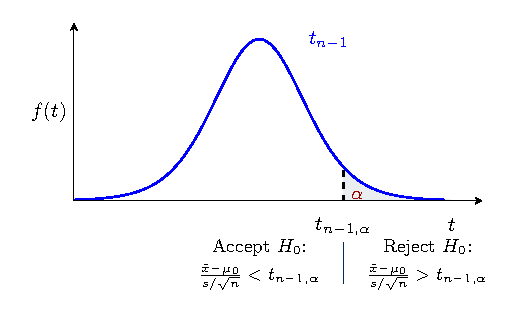
\includegraphics[clip, trim=0.5cm 0.5cm 0.0cm 0cm, width=0.95\textwidth]{Hypothesis_Testing_Module_9_t1.pdf}  
    \caption{Figure {\color{franklinblue} 12}: The Decision Rule for a Right-Tailed $H_1$ \\ for a given Significance Level $\alpha$ and Unknown $\sigma^2$}
    \label{fig:gauss4}
\end{figure}
\end{frame}

\begin{frame}[t]{$p$-value for a Right-Tailed $H_1$, $\sigma$ Unknown}
The p-values for these tests are computed in the same way as we did for tests with known variance except that the Student's $t$ value is substituted for the normal $Z$ value. \\
\vspace{1.5ex}
The $p$-value for the null hypothesis $H_0\text{: }  \mu = \mu_0$ tested against the right-tailed alternative hypothesis $H_1\text{: }  \mu > \mu_0$ is \\
\vspace{1.5ex}
\begin{equation}
p\text{-value} = P\bigg( \frac{\bar{x} - \mu_0}{s/ \sqrt{n}} \geq t_{n-1,p} | H_0\text{: }  \mu = \mu_0 \bigg),
\end{equation}
where $t_{n-1,p}$ is the $t_{n-1}$ distribution value associated with the \underline{smallest significance level} at which the null hypothesis can be rejected. \\
\vspace{1.5ex}
To obtain the $p$-value we often need to interpolate in a $t$ table or use a computer package.
\end{frame}

\begin{frame}[t]{Hypothesis Tests for $\mu$, $\sigma$ Unknown, Left-Tailed $H_1$}
\small
\begin{tcolorbox}[colback=white!5,colframe=franklinblue]%,title=A nice heading]
Suppose there is a random sample of $n$ observations from a normal distribution, $n > 30$, or the sample is approximately normal.  Let $\mu$ be the mean and variance $\sigma^2$, where $\sigma^2$ is \underline{unknown}. Given the sample standard deviation $s$, a test with significance level $\alpha$ for either of the following null hypotheses, 
\vspace{-1.0ex}
\begin{align*} 
H_0\text{: }  \mu = \mu_0 \;\; \text{ or } \;\; H_0\text{: }  \mu \;\, \textcolor{red}{\geq} \;\, \mu_0, 
\end{align*} 
\vspace{-1.0ex}
against the left-tailed composite alternative 
\vspace{0.0ex}
\begin{align*} 
H_1\text{: }  \mu \;\, \textcolor{red}{<} \;\, \mu_0, 
\end{align*} 
\vspace{-1.0ex}
is obtained by the decision rule 
\vspace{0.0ex}
\begin{equation} 
\text{Reject } H_0 \text{ if } \frac{\bar{x} - \mu_0}{s/ \sqrt{n}} \;\, \textcolor{red}{<}  -t_{n-1,\alpha},
\end{equation} 
where $-t_{n-1,\alpha}$ is the number for which $P(T < -t_{n-1,\alpha}) = \alpha$, and $T \sim t_{n-1}$. 
\end{tcolorbox}
\end{frame}

\begin{frame}[t]{Illustrating the Decision Rule for a Left-Tailed $H_1$ }
\begin{figure}[htbp]
    \centering
    \captionsetup{justification=centering}
    %\fbox{\includegraphics[trim=0cm 9cm 0cm 9cm]{../excel_pdfs/startYear_frequency_distr2.pdf}}  
    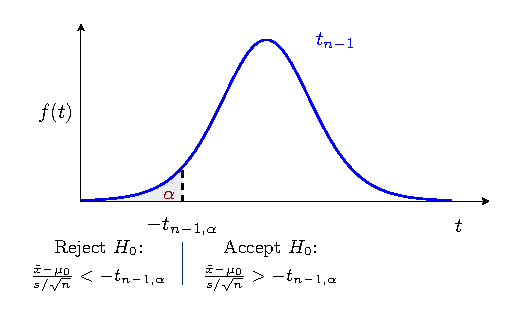
\includegraphics[clip, trim=0.5cm 0.5cm 0.0cm 0cm, width=0.95\textwidth]{Hypothesis_Testing_Module_9_t2.pdf}  
    \caption{Figure {\color{franklinblue} 13}: The Decision Rule for a Left-Tailed $H_1$ \\ for a given Significance Level $\alpha$ and Unknown $\sigma^2$}
    \label{fig:gauss5}
\end{figure}
\end{frame}

\begin{frame}[t]{$p$-value  for a Left-Tailed $H_1$, $\sigma$ Unknown}
The $p$-value for the null hypothesis $H_0\text{: }  \mu = \mu_0$ tested against the left-tailed alternative hypothesis $H_1\text{: }  \mu < \mu_0$ is \\
\vspace{1.5ex}
\begin{equation}
p\text{-value} = P\bigg( \frac{\bar{x} - \mu_0}{s/ \sqrt{n}} \leq -t_{n-1,p} | H_0\text{: }  \mu = \mu_0 \bigg),
\end{equation}
where $-t_{n-1,p}$ is the $t_{n-1}$ distribution value associated with the \underline{smallest significance level} at which the null hypothesis can be rejected. \\
\end{frame}

\begin{frame}[t]{Hypothesis Tests for $\mu$, $\sigma$ Unknown, Two-Tailed $H_1$}
\small
\begin{tcolorbox}[colback=white!5,colframe=franklinblue]%,title=A nice heading]
Suppose there is a random sample of $n$ observations from a normal distribution, $n > 30$, or the sample is approximately normal.  Let $\mu$ be the mean and variance $\sigma^2$, where $\sigma^2$ is \underline{unknown}. Given the sample standard deviation $s$, a test with significance level $\alpha$ for the null hypothesis 
\vspace{-1.0ex}
\begin{align*} 
H_0\text{: }  \mu \;\, \textcolor{red}{=} \;\, \mu_0  
\end{align*} 
\vspace{-1.0ex}
against the two-tailed composite alternative 
\vspace{0.0ex}
\begin{align*} 
H_1\text{: }  \mu \;\, \textcolor{red}{\neq} \;\, \mu_0, 
\end{align*} 
\vspace{-1.0ex}
is obtained by the decision rule 
\vspace{0.0ex}
\begin{equation} 
\text{Reject } H_0 \text{ if } \frac{\bar{x} - \mu_0}{s/ \sqrt{n}} \;\, \textcolor{red}{<} -t_{n-1,\alpha/2} \;\; \text{ or } \;\;
\frac{\bar{x} - \mu_0}{s/ \sqrt{n}} \;\, \textcolor{red}{>} \;\, t_{n-1,\alpha/2},
\end{equation} 
where $t_{n-1,\alpha/2}$ is the number for which $P(T > t_{n-1,\alpha/2}) = \alpha/2$, and $T \sim t_{n-1}$. 
\end{tcolorbox}
\end{frame}

\begin{frame}[t]{Illustrating the Decision Rule for a Two-Tailed $H_1$ }
\begin{figure}[htbp]
    \centering
    \captionsetup{justification=centering}
    %\fbox{\includegraphics[trim=0cm 9cm 0cm 9cm]{../excel_pdfs/startYear_frequency_distr2.pdf}}  
    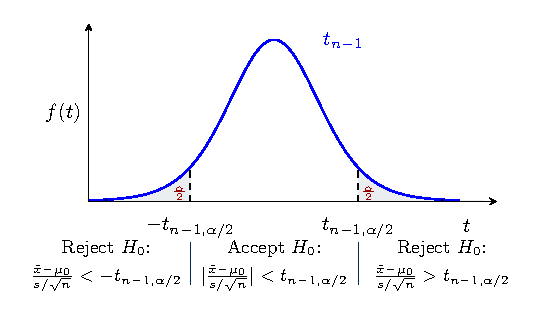
\includegraphics[clip, trim=0.5cm 0.5cm 0.0cm 0cm, width=0.95\textwidth]{Hypothesis_Testing_Module_9_t3.pdf}  
    \caption{Figure {\color{franklinblue} 14}: The Decision Rule for a Two-Tailed $H_1$ \\ for a given Significance Level $\alpha$ and Unknown $\sigma^2$}
    \label{fig:gauss6}
\end{figure}
\end{frame}

\begin{frame}[t]{$p$-value  for a Two-Tailed $H_1$, $\sigma$ Unknown}
The $p$-value for the null hypothesis $H_0\text{: }  \mu = \mu_0$ tested against the two-tailed alternative hypothesis $H_1\text{: }  \mu \neq \mu_0$ is \\
\vspace{1.5ex}
\begin{equation}
p\text{-value} = 2 \times P\bigg( \bigg| \frac{\bar{x} - \mu_0}{s/ \sqrt{n}} \bigg| \geq t_{n-1,p/2} | H_0\text{: }  \mu = \mu_0 \bigg),
\end{equation}
where $t_{n-1,p/2}$ is the $t_{n-1}$ distribution value associated with the \underline{smallest significance level} at which the null hypothesis can be rejected. \\
\end{frame}

\begin{frame}[t]{Procedure for Testing $\mu$ with $\sigma$ Unknown }
Check to be sure the assumptions are satisfied. If they are, then proceed with the following steps. \\
\vspace{1.5ex}
\begin{enumerate}
\item State the null and alternate hypotheses. A simple null hypothesis is of the form $H_0\text{: }  \mu =\mu_0$. For a simple null hypothesis, an alternate hypothesis can be stated in one of three ways:
 \begin{itemize}
  \item Right-tailed - $H_1\text{: }  \mu > \mu_0$.
  \item Left-tailed - $H_1\text{: }  \mu < \mu_0$.
  \item Two-tailed - $H_1\text{: }  \mu \ne \mu_0$.
\end{itemize}
\item Choose a significance level $\alpha$, and find the critical value or values using Student's $t$ distribution with $n-1$ degrees of freedom.
\item Compute the test statistic, $t =\frac{\bar{x} - \mu_0}{s/\sqrt{n}}$. 
\end{enumerate}
\end{frame}

\begin{frame}[t]{Procedure for Testing $\mu$ with $\sigma$ Unknown Continued}
\begin{enumerate}
  \setcounter{enumi}{3}
\item Determine whether to reject $H_0$, as follows:
 \begin{itemize}
  \item Right-tailed - $H_1\text{: }  \mu > \mu_0$; Reject $H_0$ if $t > t_{n-1,\alpha}$.
  \item Left-tailed - $H_1\text{: }  \mu < \mu_0$; Reject $H_0$ if $t < -t_{n-1,\alpha}$.
  \item Two-tailed - $H_1\text{: }  \mu \ne \mu_0$; Reject $H_0$ if $t < -t_{n-1,\alpha/2}$ or $z > t_{n-1,\alpha/2}$.
\end{itemize}
\item Find the $p$-value of the test. 
\item State a conclusion.
\end{enumerate}
\end{frame}

\section{Appendix - Hypothesis Tests for Population Proportions}

\begin{frame}[t]{Proportion Hypothesis Testing Background}
Another important set of business and economics problems involves population proportions. \\
\vspace{1.5ex}
Business executives are interested in the percent market share for their products, and government officials are interested in the percentage of people that support a proposed new program. \\
\vspace{1.5ex} 
Inference about the population proportion based on sample proportions is an important application of hypothesis testing. 
\end{frame}

\begin{frame}[t]{Proportion Hypothesis Testing Notation}
Notation: \\
\vspace{1.5ex}
\begin{itemize}
\item $p$ is the population proportion of individuals who are in a specified category. $p_0$ is the population proportion specified by the null hypothesis $H_0$.
\item $x$ is the number of sample individuals who are in the specified category.
\item $n$ is the sample size.
\item $\hat{p}$ is the sample proportion of individuals who are in the specified category:  $\hat{p} = x/n$. Frequently $\hat{p}$ is referred to as the  ``observed proportion of successes.''
\end{itemize}
\end{frame}

\begin{frame}[t]{Proportion Hypothesis Testing Assumptions}
Assumptions for large sample hypothesis testing of $p$. \\
\vspace{1.5ex}
\begin{itemize}
\item We have a simple random sample.
\item The population is at least 20 times as large as the sample.
\item The items in the population are divided into two categories.
\item The values $np_0$ and $n(1-p_0)$ are both at least 10.
\end{itemize}
\end{frame}

\begin{frame}[t, label=pRT]{Hypothesis Tests for $p$, Right-Tailed $H_1$}
\small
\begin{tcolorbox}[colback=white!5,colframe=franklinblue]%,title=A nice heading]
Suppose that the assumptions mentioned earlier in this section are met. If the observed sample proportion is $\hat{p}$, then a test with significance level $\alpha$ for either of the following null hypotheses, 
\vspace{-1.0ex}
\begin{align*} 
H_0\text{: }  p = p_0 \;\; \text{ or } \;\; H_0\text{: }  p \;\, \textcolor{red}{\leq} \;\, p_0, 
\end{align*} 
\vspace{-1.0ex}
against the right-tailed composite alternative 
\vspace{0.0ex}
\begin{align*} 
H_1\text{: }  p \;\, \textcolor{red}{>} \;\, p_0, 
\end{align*} 
\vspace{-1.0ex}
is obtained by the decision rule 
\vspace{0.0ex}
\begin{equation} 
\text{Reject } H_0 \text{ if } \frac{\hat{p} - p_0}{\sqrt{p_0(1-p_0)/ n}} \;\, \textcolor{red}{>} \;\, z_{\alpha},
\end{equation} 
where $z_{\alpha}$ is the number for which $P(Z > z_{\alpha}) = \alpha$, and $Z$ is a standard normal random variable. 
\end{tcolorbox}
\end{frame}

\begin{frame}[t]{Illustrating the Decision Rule for a Right-Tailed $H_1$ }
\begin{figure}[htbp]
    \centering
    \captionsetup{justification=centering}
    %\fbox{\includegraphics[trim=0cm 9cm 0cm 9cm]{../excel_pdfs/startYear_frequency_distr2.pdf}}  
    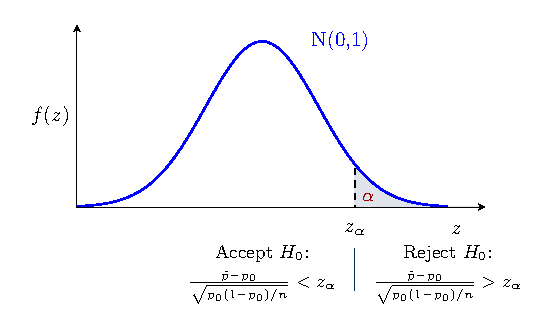
\includegraphics[clip, trim=0.5cm 0.5cm 0.0cm 0cm, width=0.95\textwidth]{Hypothesis_Testing_Module_9_pZ1.pdf}  
    \caption{Figure {\color{franklinblue} 15}: The Decision Rule for Testing $p$ with a \\Right-Tailed $H_1$ for a Given Significance Level $\alpha$}
    \label{fig:gauss7}
\end{figure}
\end{frame}

\begin{frame}[t]{$p$-value for a Right-Tailed $H_1$}
The $p$-value for the null hypothesis $H_0\text{: }  p = p_0$ tested against the right-tailed alternative hypothesis $H_1\text{: }  p > p_0$ is
\begin{equation}
p\text{-value} = P\bigg( \frac{\hat{p} - p_0}{\sqrt{p_0(1-p_0)/ n}} \geq z_{p} | H_0\text{: }  p = p_0 \bigg),
\end{equation}
where $z_p$ is the standard normal value associated with the \underline{smallest significance level} at which the null hypothesis can be rejected.
\end{frame}

\begin{frame}[t, label=pLT]{Hypothesis Tests for $p$, Left-Tailed $H_1$}
\small
\begin{tcolorbox}[colback=white!5,colframe=franklinblue]%,title=A nice heading]
Suppose that the assumptions mentioned earlier in this section are met. If the observed sample proportion is $\hat{p}$, then a test with significance level $\alpha$ for either of the following null hypotheses, 
\vspace{-1.0ex}
\begin{align*} 
H_0\text{: }  p = p_0 \;\; \text{ or } \;\; H_0\text{: }  p \;\, \textcolor{red}{\geq} \;\, p_0, 
\end{align*} 
\vspace{-1.0ex}
against the left-tailed composite alternative 
\vspace{0.0ex}
\begin{align*} 
H_1\text{: }  p \;\, \textcolor{red}{<} \;\, p_0, 
\end{align*} 
\vspace{-1.0ex}
is obtained by the decision rule 
\vspace{0.0ex}
\begin{equation} 
\text{Reject } H_0 \text{ if } \frac{\hat{p} - p_0}{\sqrt{p_0(1-p_0)/ n}} \;\, \textcolor{red}{<}  -z_{\alpha},
\end{equation} 
where $-z_{\alpha}$ is the number for which $P(Z < -z_{\alpha}) = \alpha$, and $Z$ is a standard normal random variable. 
\end{tcolorbox}
\end{frame}

\begin{frame}[t]{Illustrating the Decision Rule for a Left-Tailed $H_1$ }
\begin{figure}[htbp]
    \centering
    \captionsetup{justification=centering}
    %\fbox{\includegraphics[trim=0cm 9cm 0cm 9cm]{../excel_pdfs/startYear_frequency_distr2.pdf}}  
    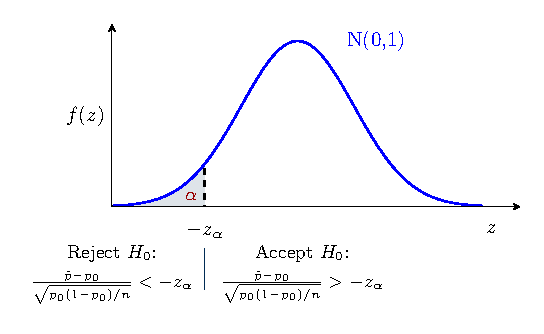
\includegraphics[clip, trim=0.5cm 0.5cm 0.0cm 0cm, width=0.95\textwidth]{Hypothesis_Testing_Module_9_pZ2.pdf}  
    \caption{Figure {\color{franklinblue} 16}: The Decision Rule for Testing $p$ with a \\ Left-Tailed $H_1$ for a given Significance Level $\alpha$}
    \label{fig:gauss8}
\end{figure}
\end{frame}

\begin{frame}[t]{$p$-value for a Left-Tailed $H_1$}
The $p$-value for the null hypothesis $H_0\text{: }  p = p_0$ tested against the left-tailed alternative hypothesis $H_1\text{: }  p < p_0$ is
\begin{equation}
p\text{-value} = P\bigg( \frac{\hat{p} - p_0}{\sqrt{p_0(1-p_0)/ n}} \leq -z_{p} | H_0\text{: }  p = p_0 \bigg),
\end{equation}
where $-z_p$ is the standard normal value associated with the \underline{smallest significance level} at which the null hypothesis can be rejected.
\end{frame}

\begin{frame}[t,label=pTT]{Hypothesis Tests for $p$, Two-Tailed $H_1$}
\small
\begin{tcolorbox}[colback=white!5,colframe=franklinblue]%,title=A nice heading]
Suppose that the assumptions mentioned earlier in this section are met. If the observed sample proportion is $\hat{p}$, then a test with significance level $\alpha$ for the null hypothesis, 
\vspace{-1.0ex}
\begin{align*} 
H_0\text{: }  p \;\, \textcolor{red}{=} \;\, p_0  
\end{align*} 
\vspace{-1.0ex}
against the two-tailed composite alternative 
\vspace{0.0ex}
\begin{align*} 
H_1\text{: }  p \;\, \textcolor{red}{\neq} \;\, p_0, 
\end{align*} 
\vspace{-1.0ex}
is obtained by the decision rule 
\vspace{0.0ex}
\begin{equation} 
\text{Reject } H_0 \text{ if } \frac{\hat{p} - p_0}{\sqrt{p_0(1-p_0)/ n}} \;\, \textcolor{red}{<} -z_{\alpha/2} \;\; \text{ or } \;\;
\frac{\hat{p} - p_0}{\sqrt{p_0(1-p_0)/ n}} \;\, \textcolor{red}{>} \;\, z_{\alpha/2},
\end{equation} 
where $z_{\alpha/2}$ is the number for which $P(Z > z_{\alpha/2}) = \alpha/2$, and $Z$ is a standard normal random variable. 
\end{tcolorbox}
\end{frame}

\begin{frame}[t]{Illustrating the Decision Rule for a Two-Tailed $H_1$ }
\begin{figure}[htbp]
    \centering
    \captionsetup{justification=centering}
    %\fbox{\includegraphics[trim=0cm 9cm 0cm 9cm]{../excel_pdfs/startYear_frequency_distr2.pdf}}  
    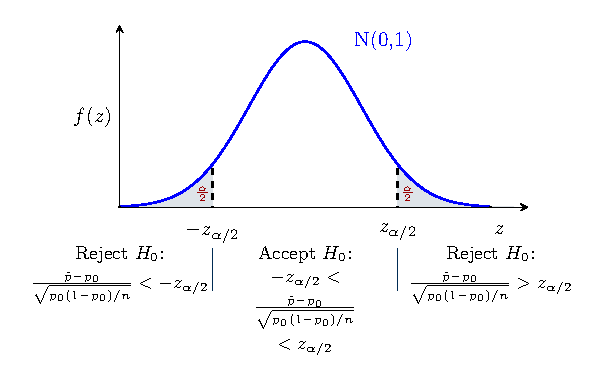
\includegraphics[clip, trim=0.5cm 0.5cm 0.0cm 0cm, width=0.95\textwidth]{Hypothesis_Testing_Module_9_pZ3.pdf}  
    \caption{Figure {\color{franklinblue} 17}: The Decision Rule for Testing $p$ with a \\ Two-Tailed $H_1$ for a given Significance Level $\alpha$}
    \label{fig:gauss9}
\end{figure}
\end{frame}

\begin{frame}[t]{$p$-value for a Two-Tailed $H_1$}
The $p$-value for the null hypothesis $H_0\text{: }  p = p_0$ tested against the two-tailed alternative hypothesis $H_1\text{: }  p \neq p_0$ is
\begin{equation}
p\text{-value} = 2 \times P\bigg( \bigg| \frac{\hat{p} - p_0}{\sqrt{p_0(1-p_0)/ n}} \bigg| \geq z_{p/2} | H_0\text{: }  p = p_0 \bigg),
\end{equation}
where $z_{p/2}$ is the standard normal value associated with the \underline{smallest significance level} at which the null hypothesis can be rejected.
\end{frame}

\begin{frame}[t]{Procedure for Testing $p$ }
Check to be sure the assumptions are satisfied. If they are, then proceed with the following steps. \\
\vspace{1.5ex}
\begin{enumerate}
\item State the null and alternate hypotheses. A simple null hypothesis is of the form $H_0\text{: }  p = p_0$. For a simple null hypothesis, an alternate hypothesis can be stated in one of three ways:
 \begin{itemize}
  \item Right-tailed - $H_1\text{: }  p > p_0$.
  \item Left-tailed - $H_1\text{: }  p < p_0$.
  \item Two-tailed - $H_1\text{: }  p \ne p_0$.
\end{itemize}
\item Choose a significance level $\alpha$, and find the critical value or values using the standard normal distribution.
\item Compute the test statistic, $z =\frac{\hat{p} - p_0}{\sqrt{p_0(1-p_0)/ n}}$.  
\end{enumerate}
\end{frame}

\begin{frame}[t]{Procedure for Testing $p$ Continued}
\begin{enumerate}
  \setcounter{enumi}{3}
\item Determine whether to reject $H_0$, as follows:
 \begin{itemize}
  \item Right-tailed - $H_1\text{: }  p > p_0$; Reject $H_0$ if $z > z_{\alpha}$.
  \item Left-tailed - $H_1\text{: }  p < p_0$; Reject $H_0$ if $z < -z_{\alpha}$.
  \item Two-tailed - $H_1\text{: }  p \ne p_0$; Reject $H_0$ if $z < -z_{\alpha/2}$ or $z > z_{\alpha/2}$.
\end{itemize}
\item Find the $p$-value of the test. 
\item State a conclusion.
\end{enumerate}
\end{frame}

\end{document}